



\section{Day ahead and real time energy prices} \label{sec:day_ahead_and_real_time_energy_prices}

A system comprising a day ahead as well as a real time market is also known as two-settlement system \cite{lambert2001creating}. Day ahead and real time markets are classified as short-term markets within the scope of deregulated wholesale power markets \cite{hogan1993competitive}. 
%A two settlement system has been defined for the PJM power market (PJM standing for Pennsylvania, New Jersey, Maryland)\cite{lambert2001creating}. 

In day ahead or spot markets bids are placed for each consecutive hour of the following day. Prices may change substantially from one hour to the next, up to a factor of ten \cite{huisman2007hourly,weron2004modeling}. Therefore market operators need to apply profound risk management techniques to alleviate such price spikes.

The real time market, also called intraday or balancing market on the other hand is used to compensate demand variations during the day which may result in additional changes in energy prices \cite{barroso2005classification}. 
Due to this characteristic the real time market prices exhibit an even greater volatility than those of the day-ahead market. 

A direct comparison of day ahead and real time prices is depicted in Figure \ref{fig:da_vs_rt_prices_maine}.

\begin{figure}[!htbp]
	\centering
		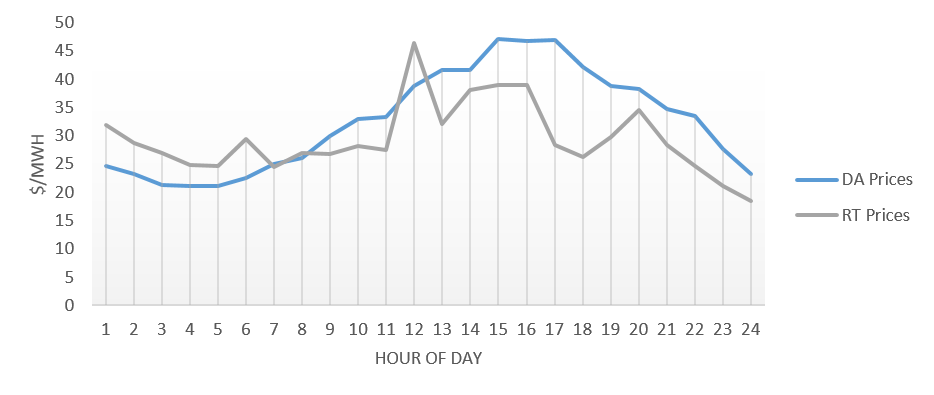
\includegraphics[width=0.90\textwidth]{figures/data_analysis/day_ahead_vs_real_time_prices.png}
	\caption{Day ahead vs real time energy prices, Maine 4th Aug, 2015}
	\label{fig:da_vs_rt_prices_maine}
\end{figure}

What can be noted is that both day ahead and real time prices show a clear trend over one day denoting a daily seasonality pattern, with real time prices exhibiting more variation during the day. Thus prices start to rise at 5 a.m.~and start falling again at around 5 p.m. This pattern is highly related to energy demand which reaches its peak during the day mainly due to industrial power demands. 

Price time series spanning a whole month can be seen in Figure \ref{fig:da_rt_prices_aug_2015}. It shows day ahead and real time markets (top to bottom) from Portland, Maine belonging to the ISO New England power market which is located in Northeast USA. It covers the whole month of August 2015 to display energy price characteristics over an extended time range. 
Some characteristics of energy prices can be spotted in both day ahead and real time markets such as daily and weekly seasonality, trends, price volatility and price spikes (see Section \ref{sec:characteristics_of_energy_markets}). 

Daily and weekly seasonality are most evident in day ahead markets. Apart from the daily variations of energy prices a weekly seasonality is clearly visible where prices are higher at the start of a week and decline towards the end of the week. This may be explained by the fact that power demand is most present at the start of the week and is usually decreased on weekends due to the weekly lifecycle of industrial facilities and established companies. Even though the real time market shows much higher volatility in energy price levels the daily and weekly seasonality are still present. 

Price trends can be observed during the second week of this investigation where prices continuously rise and hit a peak at the beginning of the third week. Weekly seasonality might therefore be masked by the increasing trend however it can still be spotted as the price peak of the second day is surpassed by the one of the previous day. In the third and fourth weeks prices continue to decline to return to their former levels. 

\begin{figure}[htbp]
	\centering
		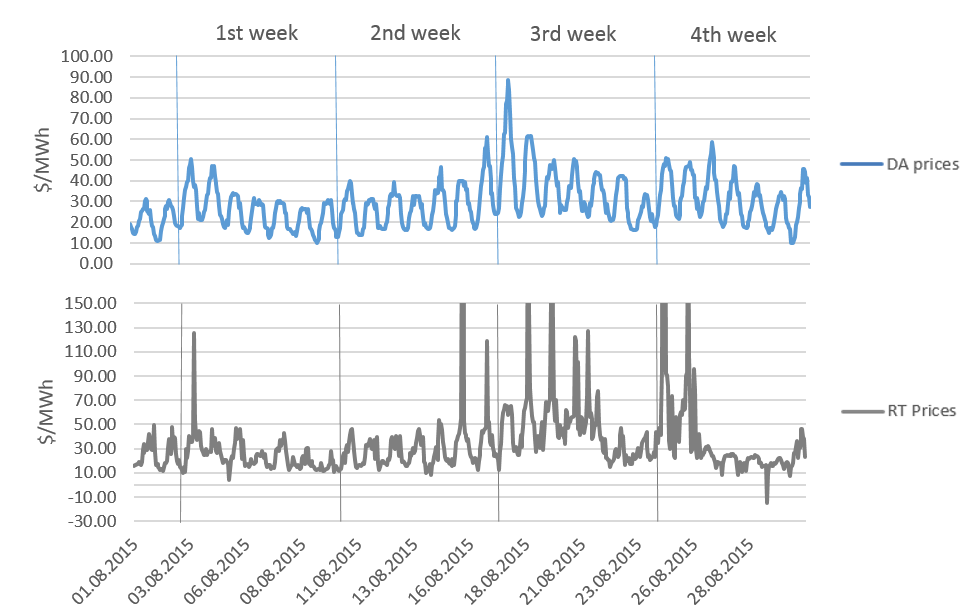
\includegraphics[width=0.95\textwidth]{figures/data_analysis/da_rt_prices_aug_2015.png}
	\caption{Day ahead and real time prices, ISO-NE, ME}
	\label{fig:da_rt_prices_aug_2015}
\end{figure}

Price volatility is most evident in the real time market where variations in energy price levels is more common than in the corresponding day ahead market. Seasonality is less clear and prices tend to change their levels more often and to a greater extent than those at the day ahead market. This can be observed in the middle of the third week where prices experience a sudden drop in price level and variation. 

An important characteristic of energy prices in deregulated markets are the so called \textit{price spikes} \cite{weron2004modelingmarkets}. A price spike is defined as an extreme price increase (more than three times the standard deviation of the price series) from one observation time stamp to the next where the price tends to rapidly return to its normal level again. 
A price spike appears e.g.~when there is a sudden surge in power demand or a power outage occurred. In the lower part of Figure \ref{fig:da_rt_prices_aug_2015} the real time market shows several price spikes. Major spikes can be observed on the 15th, 18th, 19th, 24th and 25th of August. As the spikes reached maximum values of up to \$ 700 the range of the y axis has been limited to be able to accurately observe relevant price characteristics. 

Another more subtle characteristic of energy prices in wholesale power markets is the occurrence of negative prices. This phenomenon can occur when an excess of electricity is produced which cannot be easily distributed to consumers as electricity demand is low. In this situation market participants are actually paid to get electricity from the market in order to stabilize supply and demand. As electricity is not storable at a larger scale it has to be consumed as soon as it is produced. 
In Figure \ref{fig:da_rt_prices_aug_2015} a negative price occurs at the end of the fourth week on the 28th of August where prices and demand tend to be low which finally leads to a small negative price spike. 



\section{Characteristics of energy markets} \label{sec:characteristics_of_energy_markets}

In this section different studies of power market characteristics are presented to distinguish features that may be used in building forecasting models. 


The main differences between electricity power markets and other financial markets are price volatility, mean reversion and price jumps or "`spikes"' \cite{weron2007modeling,weron2008market,weron2004modelingmarkets}. In addition to these characteristic features electricity prices may exhibit strong seasonality patterns on a daily, weekly and annual basis \cite{weron2004modelingmarkets}. 

Volatility and price variations are inherent characteristics of deregulated power markets as energy cannot be stored but has to be delivered immediately. This results in constant balancing of electricity demand vs.~supply to ensure the stability of the electrical grid which has a direct impact on energy prices. When building energy price models the impact of price variations can be reduced by applying logarithmic transformations to input data or utilizing Box Cox transformations \cite{weron2005forecasting, box1964analysis}. 

Energy prices in general exhibit strong mean reversion which denotes the characteristic that prices tend to return to their mean levels after a significant deviation from the mean \cite{weron2004modelingmarkets,weron2007modeling}. To discover mean reversion or long range dependencies in time series different models can be utilized of which the most important are rescaled range analysis, Detrended Fluctuation Analysis, periodogram regression and Average Wavelet Coefficient \cite{weron2007modeling}. By applying these methods to electricity price data strong mean reversion could be detected in contrast to typical financial stock indices where this behavior can not be recognized. 


Price jumps or spikes are a distinctive feature of electricity markets due to the non-storable nature of electricity prices and occasional gaps in supply vs.~demand caused by transmission congestion, plant failure or unanticipated high power consumption \cite{weron2004modelingmarkets, weron2007modeling}. 
Considering price spikes is critical as price values may increase tenfold from one hour to the next \cite{huisman2007hourly}. 
These phenomenons are called spikes as prices tend to rapidly return to their previous level after the sudden increase. In order to model price spikes a combination of mean reversion and "`downward jumps"' can be applied. Another possibility is to model positive and negative jumps through the application of \textit{jump diffusion models} \cite{weron2004modeling}. These kind of models are able to accurately model price spikes. 

The actual root cause of price spikes lies in the applied bidding strategy (Section \ref{ssec:bidding_strategies}) \cite{weron2007modeling}. Since electricity is an essential commodity for most market participants they are willing to pay almost any price to ensure a continuous supply of electric power. Thus bids on demand side are regularly placed at the highest possible price (price cap) which results in suppliers raising their bids as well since they are aware of these bidding strategies. Since bids are placed for all 24 hours of the following day market participants have to stick with high priced periods for at least one day before they can choose to search for cheaper alternatives. 



%Electricity wholesale markets are constantly developing. In Europe incentives exist to create an integrated EU energy market for secure and affordable electricity supplies\footnote{\url{https://ec.europa.eu/energy/en/topics/markets-and-consumers}}. Also concrete plans exist for creating a so called \emph{Energy Union} as a single energy market that aim to make energy more reliable and interchangable within the EU\footnote{\url{https://ec.europa.eu/energy/en/news/new-electricity-market-consumers}}. 

An outline of a possible implementation of a competitive energy market is depicted in \cite{hogan1993competitive} which is still valid as of today in many respects. A competitive market captures the advantage of market participants being able to actively shaping the final clearing price applicable to both producers and consumers in the market. Thus the market price more accurately resembles actual market conditions in contrast to a defined price dictated in regulated markets. 




\subsection{Electricity market models}

Two main models exist for the exchange and types of trading of energy prices in power markets which are bilateral trading and electricity pooling, also called loose pool and tight pool models \cite{onaiwu2009does,hogan1997reshaping,barroso2005classification,chao1999design}.

\subsubsection{Bilateral trading}

In bilateral trading or loose pool models utility operators (producers) and energy consumers establish bilateral contracts to determine the terms and conditions applied for trading energy \cite{onaiwu2009does,chao1999design}. Generators or producers may also buy electricity from other suppliers in case their own electricity generation does not fit current demand. The exact amount, price and time when tradings take place are negotiated on the contract. Since electricity demand may vary from the negotiated terms the resulting imbalances have to be taken care of by the system operator. 

\subsubsection{Electricity pooling}

Electricity pooling in tight pool models provide a way for utility operators to offer a certain amount of energy at a set price. Each generator places a bid containing the quantity and expected price \cite{barroso2005classification}. In return consumers place bids on how much they are willing to pay for a given amount of energy. The intersection of the aggregated demand and supply curves defines the energy price for that hour. 
Customers, brokers and aggregators have the choice to either establish long term contracts of electricity in bilateral contracts or rely on the short-term market \cite{hogan1997reshaping}.



\subsubsection{Forward Capacity Market (FCM)} 

In contrast to day ahead and real time markets which are classified as short term markets (Section \ref{sec:day_ahead_and_real_time_energy_prices}) other types of markets exist for mid- and long term planning to ensure sufficient capacities over an extended period of time \cite{barroso2005classification,nomikos2010modelling,redl2009price}. One of the most important of these markets is the Forward Capacity Market which is introduced shortly. 

A forward capacity market is used to ensure having enough capacity for a specific amount of time into the future \cite{gottstein2010role}. A capacity commitment period (CCP) ensures that a certain amount of capacity will be available during that period. For example, the CCP at ISO-NE is set as one year ranging from June 1st until May 31st. 

The market has to ensure that the \emph{Installed Capacity Requirements (ICR)} for the corresponding region are met. These requirements are defined for each capacity commitment period and define the amount of capacity needed to meet estimated peak and reserve demands. Important measures to define the ICR are the local sourcing requirements (LSR) and maximum capacity limits (MCL) that define the constraints given by market participants. 

The actual procurement of resources for each capacity commitment period is determined by a \emph{Forward Capacity Auction (FCA)} which aims to meet the defined ICRs for the given period.
This auction is carried out three years ahead of the related CCP to ensure that enough resources will be available during that period. \emph{Reconfiguration Auctions (RA)} are then executed annually until the start of the CCP and continued monthly afterward. During an RA capacity resources may be amended to adapt to potential changes in capacity zones \cite{gottstein2010role}. 

At the FCM of ISO New England there is also the option of making a composite offer where different capacity resources may join their capacity offers (useful e.g.~in case of single season capacities) to result in a single resource offer at the market. 



\subsection{Power pools vs power exchanges}

Two types of power markets have been established, power pools and power exchanges. The main difference between those types is the type of auction that is applied. In power pools one sided auctions are conducted whereas in power exchanges two sided auctions are performed \cite{weron2007modeling}. The difference lies in the fact whether demand bids are conducted for each hour of the following day or power demand is estimated based on current demand in the market. 

\begin{figure}[htbp]
	\centering
		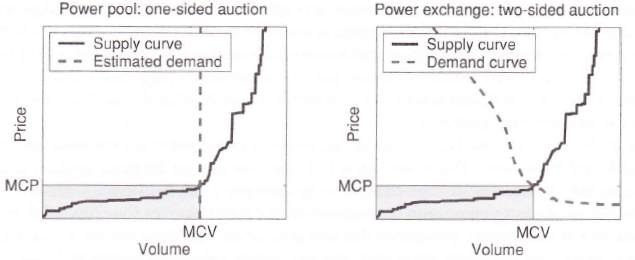
\includegraphics[width=0.8\textwidth]{figures/data_analysis/power_markets_one_two_sided_auctions.PNG}
	\caption{One sided and two sided auctions in power markets \cite{weron2007modeling}}
	\label{fig:power_markets_one_two_sided_auctions}
\end{figure}

The market clearing price (MCP) is the final settled price that results from demand and/or supply bids for a specific hour of the following day. This price can be taken as reference price for the corresponding hour that is to be paid by consumers. The market clearing volume (MCV) is the estimated energy demand (volume) for the corresponding hour that is to be generated by suppliers \cite{weron2007modeling}. 

For one sided auctions power demand is estimated for all consumers for one specific hour which results in the market clearing volume. The market clearing price is determined by the intersection between the supply curve (consisting of aggregated supply bids) and the market clearing volume. 
For two sided auctions the demand curve is established by aggregated demand bids and the MCP is determined by the intersection between the supply and demand curves (Figure \ref{fig:power_markets_one_two_sided_auctions}) \cite{weron2007modeling}. 

The sudden increase in slope of the supply price curve indicates that when market volume reaches a certain threshold a significantly higher price has to be paid due to the activation of more expensive power generation utilities. For example, a market area may depend on renewable energy (hydro generation utilities, wind turbines) for times with low electricity demand, however additional gas and coal power plants may need to be activated when electricity demand increases. 

All power markets considered in this work are part of the category \textit{power exchanges} and thus conduct two sided auctions. The following markets have been investigated: Nord Pool Spot, EPEXSpot, Belpex, ISO New England, PJM (Pennsylvania, New Jersey, Maryland). Despite its name, \textit{Nord Pool Spot} is not a power pool but is considered a power exchange. 


\subsection{Bidding strategies} \label{ssec:bidding_strategies}

In deregulated power markets two bidding strategies have evolved over time, pay-as-bid and uniform pricing \cite{weron2007modeling,tierney2008uniform}. In \cite{tierney2008uniform} it is discussed why pay-as-bid models are not necessarily more cost effective than uniform pricing models even though they seem to offer greater benefits at the first glance. 

\subsubsection{Pay-as-bid model}

In a pay-as-bid auction suppliers place bids according to the desired compensation (\$ per MWh) for quantities sold in the market \cite{tierney2008uniform}. Suppliers are paid exactly the amount they bid for the quantity transacted, there is no uniform market price which applies to all market participants. Therefore suppliers aim to maximize their revenue by placing bids more closely to the expected average bid price such that they "`win"' a greater amount of offers. An offer is won when a bid is placed at or below the offer price of the last bidder whose supplies are needed to meet customer demand. 

\subsubsection{Uniform pricing model}

In contrast to a pay-as-bid model the uniform pricing model demands suppliers to place bids that reflect their actual marginal costs rather than a desired compensation \cite{tierney2008uniform}. Supply bids are ranked according to their bid prices, such that supplies exhibiting the least costs are considered first. Suppliers are then dispatched in this order until the total customer demand is met. The supply bid of the last considered supplier is set as the uniform market clearing price that has to be paid by all market participants which placed demand bids at or above the market clearing price. 

\subsection{Electricity price characteristics in European Power Markets}

In \cite{mugele2005stable} different European power markets have been investigated to reveal major differences in energy price behaviour. The EEX, Nord Pool Spot and Polish power markets have been evaluated whereby the markets are responsible for the Mid-Europe, Northern Europe and Polish regions respectively. 

As electricity prices depend on energy demand which changes due to climate conditions (temperature and number of daylight hours) electricity prices exhibit a seasonal component as well (Figure \ref{fig:seasonal_behaviour_of_eex_prices}) \cite{weron2005forecasting}. 

\begin{figure}[htbp]
	\centering
		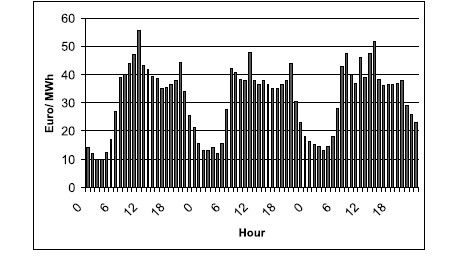
\includegraphics{figures/state_of_the_art/seasonal_behaviour_of_eex_prices.PNG}
	\caption{EEX - hourly spot prices \cite{mugele2005stable}}
	\label{fig:seasonal_behaviour_of_eex_prices}
\end{figure}

The daily seasonality for hourly spot prices at EEX (Figure \ref{fig:seasonal_behaviour_of_eex_prices}) can be clearly spotted where prices 
start rising at 6 a.m.~to 8 a.m.~and begin to fall at around 10 p.m. Daily variations of prices are caused by reduced electricity demand and power consumption at nights. 

Even though price seasonality and trend seem to be stable over a short time range (Figure \ref{fig:seasonal_behaviour_of_eex_prices}) they can show significant fluctuations over a longer time range. In \cite{mugele2005stable} data related to each examined energy market was fitted to a stable Paretian distribution as well as a normal distribution. The result showed that mature markets as EEX or Nord Pool Spot exhibit high volatility, heavy tails, high kurtosis and asymmetrics in the energy price data which was best modeled by the Paretian distribution. In contrast the Gielda Energii SA market in Poland shows a much more stable energy price behavior which can be modeled by a Gaussian distribution. 

The variation in energy price levels for the two power markets EEX and Nord Pool Spot are shown in Figures \ref{fig:EEX_levels} and \ref{fig:NordPool_levels}.

\begin{figure}[!htbp]
  \centering
  \begin{minipage}[b]{0.4\textwidth}
    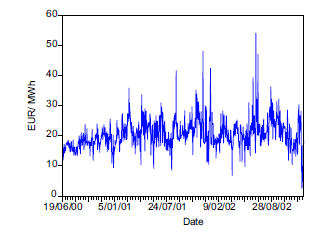
\includegraphics[width=\textwidth]{figures/state_of_the_art/EEX_levels.PNG}
    \caption{EEX levels \cite{mugele2005stable}}
		\label{fig:EEX_levels}
  \end{minipage}
  \hfill
  \begin{minipage}[b]{0.4\textwidth}
    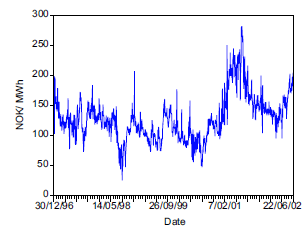
\includegraphics[width=\textwidth]{figures/state_of_the_art/NordPool_levels.PNG}
    \caption{Nord Pool levels \cite{mugele2005stable}}
		\label{fig:NordPool_levels}
  \end{minipage}
\end{figure}

By comparing these graphs by scale over a longer period of time (150 NOK equal to about 20 Euros in 2002) it is clearly visible that both energy price levels and amount of price variation can be very different across power markets. 


\section{Energy price case study}

In this section the aforementioned characteristics of electricity prices in power markets will be investigated for both day ahead and real time energy price data over an extended range of time. 


\subsection{Evaluation of electricity market price characteristics}

Through display of energy price time series over an extended time range the general behavior of different energy markets can be observed. Day ahead and real time energy price time series have been collected for the years 2012 to 2014 which are displayed in figures \ref{fig:da_energy_markets_2012_2014} and \ref{fig:rt_energy_markets_2012_2014}. 

The title displays the name of the energy market followed by the country abbreviation and an indicator whether this market is a day ahead or real time market (DA or RT). Strongest price variations are experienced in real time markets (Figure \ref{fig:rt_energy_markets_2012_2014}) where price spikes of almost 2000 \$/MWh occur. 


\begin{figure}[htbp]
	\centering
		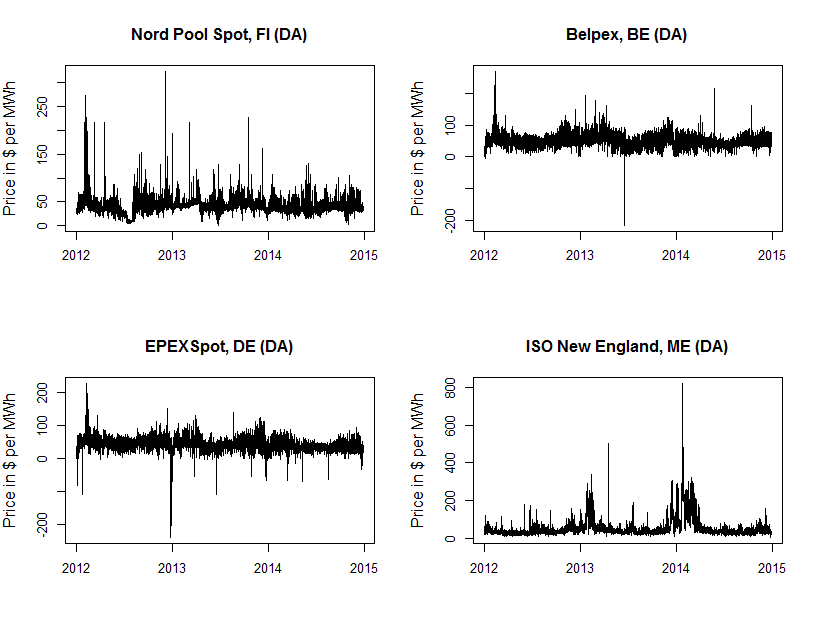
\includegraphics[width=0.8\textwidth]{figures/data_analysis/da_energy_markets_2012_2014.png}
	\caption{Day ahead energy market prices}
	\label{fig:da_energy_markets_2012_2014}
\end{figure}

\begin{figure}[htbp]
	\centering
		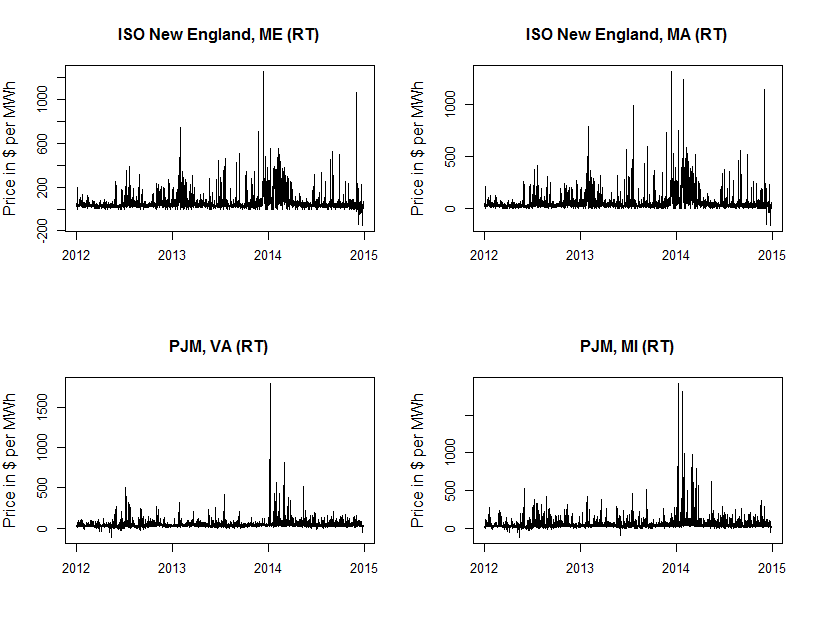
\includegraphics[width=0.8\textwidth]{figures/data_analysis/rt_energy_markets_2012_2014.png}
	\caption{Real time energy market prices}
	\label{fig:rt_energy_markets_2012_2014}
\end{figure}

What can be noted is that markets Belpex and EPEXSpot appear to be the most stable in terms of energy price level and variations except some occasional negative spikes throughout the dataset. The aggregated statistics for each market are outlined in tables \ref{table:day_ahead_market_summary} and \ref{table:real_time_market_summary}. 

The inter quartile range (range between 1st quartile and 3rd quartile) of the market prices lies between 20 \$/MWh and 60 \$/MWh whereas the minimum and maximum values tend to lie far outside this range. Real time markets exhibit significantly greater values for skewness and kurtosis which indicates a higher probability of extreme price spikes. When comparing maximum price values of real time markets to those of day ahead markets this fact is supported as well. 
The stable variability of Belpex and EPEXSpot is also emphasized through a low absolute value for the skewness which indicates an almost symmetrical distribution. In contrast, other markets are heavy tailed and experience far more "`outliers"' indicated by a higher value for skewness. 



%%%%%%%%%%%%%%%%%%%%%%%%%%%%%%%%%%%%%%%%%%%%%%%%%%%%%%
%%%%%%%%%% Skewness and kurtosis explanation %%%%%%%%%
%%%%%%%%%%%%%%%%%%%%%%%%%%%%%%%%%%%%%%%%%%%%%%%%%%%%%%

%Skewness quantifies how symmetrical the distribution is.
%
%•	A symmetrical distribution has a skewness of zero.
%•	An asymmetrical distribution with a long tail to the right (higher values) has a positive skew.
%•	An asymmetrical distribution with a long tail to the left (lower values) has a negative skew.
%•	The skewness is unitless.
%•	Any threshold or rule of thumb is arbitrary, but here is one: If the skewness is greater than 1.0 (or less than -1.0), the skewness is substantial and the distribution is far from symmetrical.
%Kurtosis quantifies whether the shape of the data distribution matches the Gaussian distribution.
%
%•	A Gaussian distribution has a kurtosis of 0.
%•	A flatter distribution has a negative kurtosis,
%•	A distribution more peaked than a Gaussian distribution has a positive kurtosis.
%•	Kurtosis has no units.
%•	The value that Prism reports is sometimes called the excess kurtosis since the expected kurtosis for a Gaussian distribution is 0.0.
%•	An alternative definition of kurtosis is computed by adding 3 to the value reported by Prism. With this definition, a Gaussian distribution is expected to have a kurtosis of 3.0.
%
%http://www.graphpad.com/guides/prism/6/statistics/index.htm?stat_skewness_and_kurtosis.htm


%> xtable(da_statistics)
% latex table generated in R 3.1.1 by xtable 1.8-2 package
% Mon Mar 14 05:40:05 2016
\begin{table}[ht]
\centering
\begin{tabular}{rrrrrrrrr}
  \hline
 & Min & 1st Qu. & Median & Mean & 3rd Qu. & Max & Skew. & Kurt. \\ 
  \hline
NPS, FI (DA) & 1.49 & 33.08 & 39.18 & 40.91 & 46.33 & 324.00 & 3.60 & 40.02 \\ 
  Belpex, BE (DA) & -216.00 & 37.14 & 48.60 & 48.66 & 59.49 & 270.00 & 0.08 & 13.35 \\ 
  EPEXSpot, DE (DA) & -239.70 & 31.20 & 39.34 & 40.73 & 51.16 & 226.80 & -1.06 & 25.29 \\ 
  ISO NE, ME (DA) & 3.00 & 28.94 & 37.18 & 50.78 & 50.41 & 817.70 & 3.62 & 23.62 \\ 
   \hline
\end{tabular}
\caption{Day ahead energy market summary statistics}
\label{table:day_ahead_market_summary}
\end{table}
%> xtable(rt_statistics)
% latex table generated in R 3.1.1 by xtable 1.8-2 package
% Mon Mar 14 05:40:06 2016
\begin{table}[ht]
\centering
\begin{tabular}{rrrrrrrrr}
  \hline
 & Min & 1st Qu. & Median & Mean & 3rd Qu. & Max & Skew. & Kurt. \\ 
  \hline
ISO NE, ME (RT) & -147.00 & 26.42 & 34.83 & 49.21 & 48.90 & 1257.00 & 4.24 & 42.21 \\ 
  ISO NE, MA (RT) & -153.90 & 27.24 & 35.99 & 52.23 & 50.92 & 1310.00 & 4.76 & 48.87 \\ 
  PJM, VA (RT) & -118.60 & 26.33 & 30.34 & 35.85 & 36.93 & 1789.00 & 24.53 & 996.02 \\ 
  PJM, MI (RT) & -120.80 & 27.76 & 32.82 & 43.83 & 41.52 & 1913.00 & 14.12 & 316.98 \\ 
   \hline
\end{tabular}
\caption{Real time energy market summary statistics}
\label{table:real_time_market_summary}
\end{table}


In order to visualize the aforementioned statistical properties histograms have been generated for each market over the whole time range (Figures \ref{fig:Histograms_da_2012_2014} and \ref{fig:Histograms_rt_2012_2014}). 

As outlined before the Belpex and EPEXSpot markets exhibit the most stable distribution of prices which is visible in the histograms as these markets show the most symmetric distributions. They exhibit an almost gaussian like distribution whereas other markets are clearly heavy tailed to the right. In order to see the distribution of prices more distinctly the histograms where cut off at 250 \$/MWh to be able to accurately compare the price distributions. 

The previously shown results have major implications for the generation of forecasting models. Various models have different requirements regarding statistical properties of the data, for example statistical time series models demand a constant mean and variance in the dataset to capture the underlying time series characteristics. When observing the discussed energy price time series these characteristics can not be found for any time series over an extended period of time. Therefore, in order to accurately model energy prices data preprocessing steps have to be taken before applying statistical models. An in-depth discussion about forecasting models and data preprocessing is provided in Chapter \ref{ch:forecasting}. 



\begin{figure}[htbp]
	\centering
		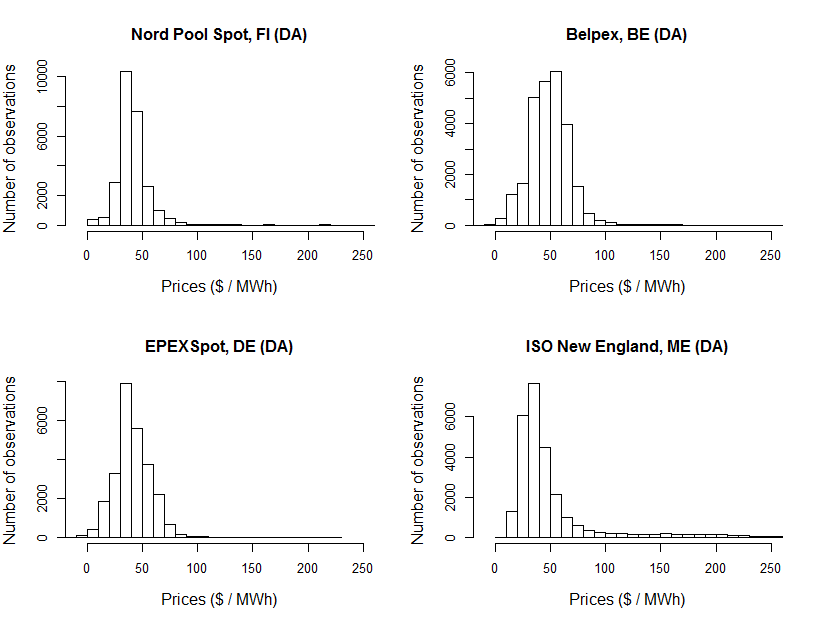
\includegraphics[width=0.8\textwidth]{figures/data_analysis/Histograms_da_2012_2014.png}
	\caption{Histograms of day ahead markets for years 2012 to 2014}
	\label{fig:Histograms_da_2012_2014}
\end{figure}

\begin{figure}[htbp]
	\centering
		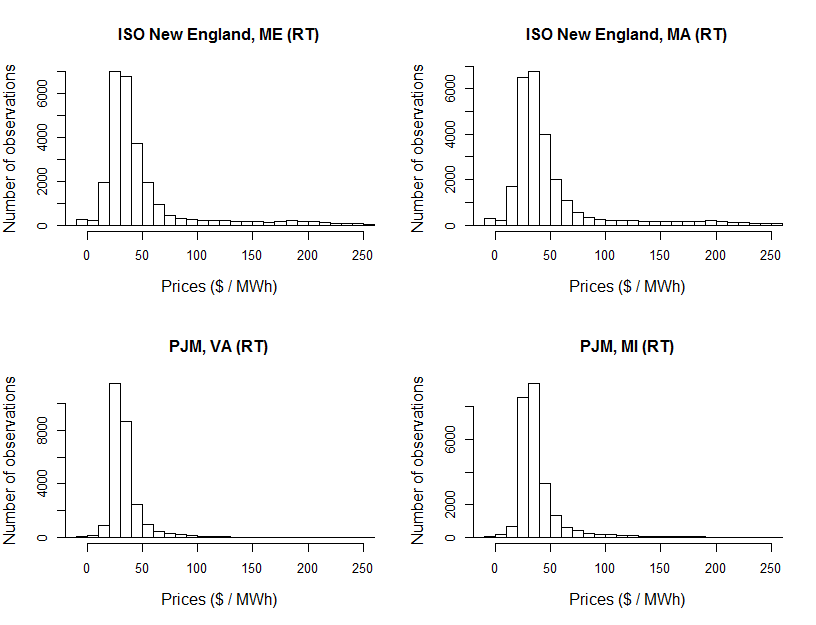
\includegraphics[width=0.8\textwidth]{figures/data_analysis/Histograms_rt_2012_2014.png}
	\caption{Histograms of real time markets for years 2012 to 2014}
	\label{fig:Histograms_rt_2012_2014}
\end{figure}




